\noindent Considérons toujours un \texttt{MDP} avec :
\begin{itemize}[label=\textbullet]
    \item des états $s\in S$
    \item des actions $a\in A$
    \item un modèle $T(s,a,s')$
    \item une fonction de récompense $R(s,a,s')$
\end{itemize}
Nous sommes toujours à la recherche d'une politique $\pi(s)$. Cependant, nous ne connaissons plus pour autant le modèle ni la
fonction de récompense. Le but est d'apprendre quelles actions prendre dans quel état pour maximiser la récompense. Un schéma
qu'il faut avoir en tête est le suivant :
\begin{figure}[H]
    \centering
    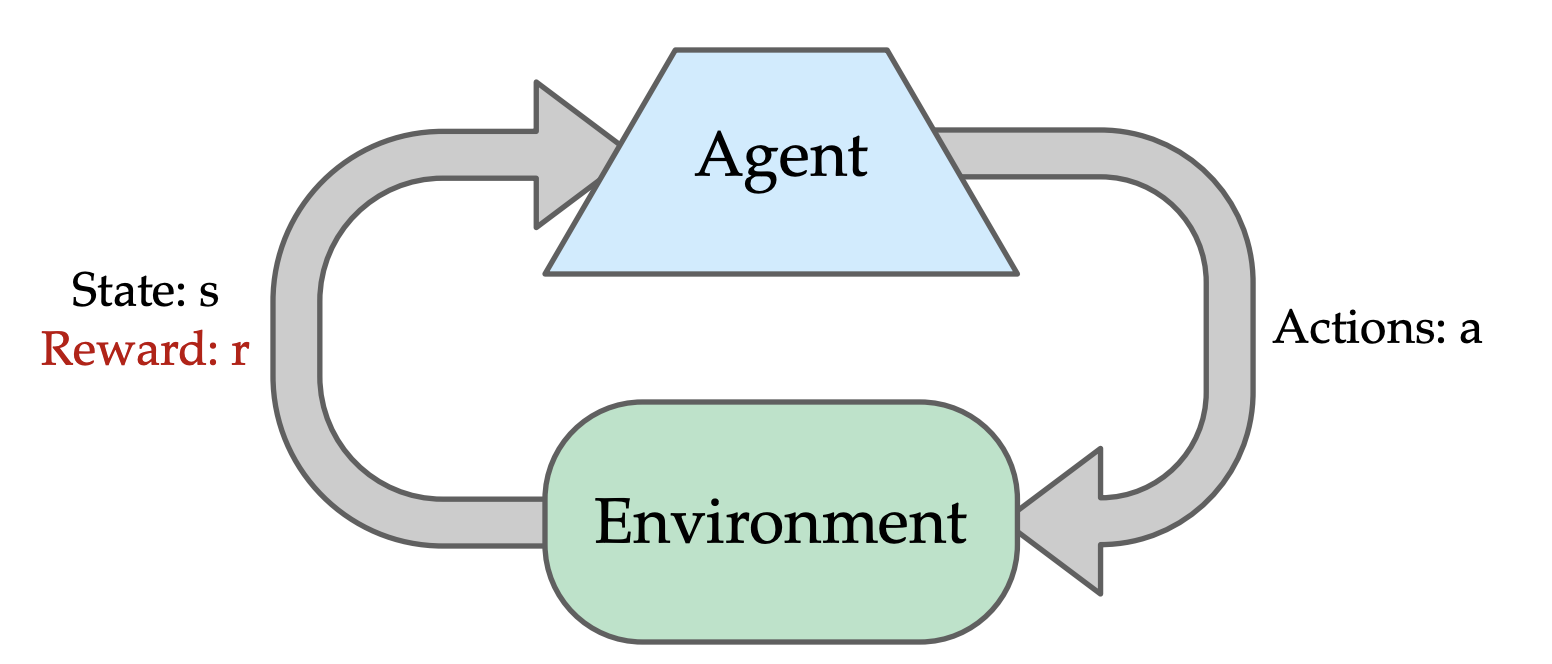
\includegraphics[width=0.5\linewidth]{pictures/rl_scheme.png}
    \caption{Schéma de l'apprentissage par renforcement}
    \label{fig:rl_scheme}
\end{figure}
\noindent L'idée est la suivante :
\begin{itemize}[label=\textbullet]
    \item On reçoit un feedback de l'environnement (reward).
    \item L'utilité de l'agent est définie par la fonction de récompense.
    \item L'agent doit apprendre à maximiser les récompenses attendues.
    \item Tous l'apprentissage est basé sur des observations d'output de l'environnement.
\end{itemize}

\subsection{Passive Reinforcement Learning} % (fold)
Nous parlons de passive RL car nous avons une politique fixe $\pi(s)$, nous ne connaissons pas les transitions $T(s,a,s')$ ni
les récompenses $R(s,a,s')$. Dans le cas du passive RL, on ne choisit pas les actions prises, on exécute simplement la politique
et nous apprenons via l'expérience.
\warningbox{
    Ce n'est pas \texttt{OFFLINE} car l'apprenant prend des actions dans le monde.
}
\subsubsection{Model-based Passive RL} % (fold)
\label{ssub:model_based_passive_rl}
\begin{definition}{Model-based Passive RL}{}
    Le but est d'apprendre le modèle MDP depuis les expériences et ensuite de résoudre le MDP appris.
\end{definition}
Le model-based RL est donc divisé en deux étapes :
\begin{enumerate}
    \item Apprendre le modèle MDP empirique 
    \begin{enumerate}
        \item Compter les résultats $s'$ pour chaque transition $(s,a)$.
        \item Normaliser afin de donner une estimation $\hat{T}(s,a,s')$.
        \item Découvrir chaque $\hat{R}(s,a,s')$ quand on fait $(s,a,s')$.
    \end{enumerate}
    \item Résoudre le MDP appris, en utilisant par exemple la value iteration.
\end{enumerate}
\begin{example}
    Imaginons que notre but est de prédire l'age des étudiants en informatique. Nous avons vu précédemment comment trouver 
    ceci grâce à l'équation suivante :
    \begin{equation*}
        E[A] = \sum_{a}P(a)\cdot a
    \end{equation*}
    Maintenant, imaginons qu'on ait pas $P(A)$, on pourrait alors récolter un tas d'échantillons $[a_1,a_2,\dots,a_n]$ et
    voici la différence entre l'approche \textit{model based} et \textit{model free} :\\
    \noindent\begin{minipage}{.5\linewidth}
    \begin{equation*}
        \textbf{model-based}\rightarrow E[A] \approx \sum_{a} \hat{P}(a)\cdot a | \hat{P}(a) = \frac{\text{count}(a)}{n}
    \end{equation*}
    \end{minipage}
    \begin{minipage}{.5\linewidth}
        \begin{equation*}
            \textbf{model-free}\rightarrow E[A] \approx \frac{1}{n}\sum_{i}a_i
        \end{equation*}
    \end{minipage}
    Le $\hat{P}(a)$ du \textit{model-based} est éventuellement le bon modèle et c'est pour cela que ça fonctionne.
\end{example}

\subsubsection{Model-free Passive RL} % (fold)
\label{ssub:model_free_passive_rl}
\begin{definition}{Model-free Passive RL}{}
    Renoncer à l'apprentissage du modèle MDP et apprendre directement la fonction de valeur $V$ ou $Q$.\\
    \begin{itemize}[label=\textbullet]
        \item $V$ fait référence à value learning où on apprend la valeur d'une politique fixe. Elle est constituée
        de deux approches : l'\textbf{évalutation directe}(cf.\ref{ssubsub:direct_evaluation}) et le \textbf{TD learning}
        (cf.\ref{ssubsub:td_learning}).
        \item $Q$ fait référence à Q-learning où on apprend les Q-valeurs de la politique optimale. L'approche utilisée
        est une Q-version du TD learning.
    \end{itemize}
\end{definition}

\subsubsubsection{Direct evaluation} % (fold)
\label{ssubsub:direct_evaluation}
Le \textbf{but} est de calculer les valeurs pour chaque état sous la politique $\pi$. L'\textbf{idée} est de faire la moyenne
de l'ensemble des valeurs observées de l'échantillon, pour ce faire :
\begin{itemize}[label=\textbullet]
    \item On agit par rapport à la politique $\pi$.
    \item A chaque fois qu'on visite un état, on met à jour la somme des récompenses.
    \item On fait la moyenne sur beaucoup d'échantillons.
\end{itemize}
\begin{example}
    Voici un exemple de direct evaluation :
    \begin{figure}[H]
        \centering
        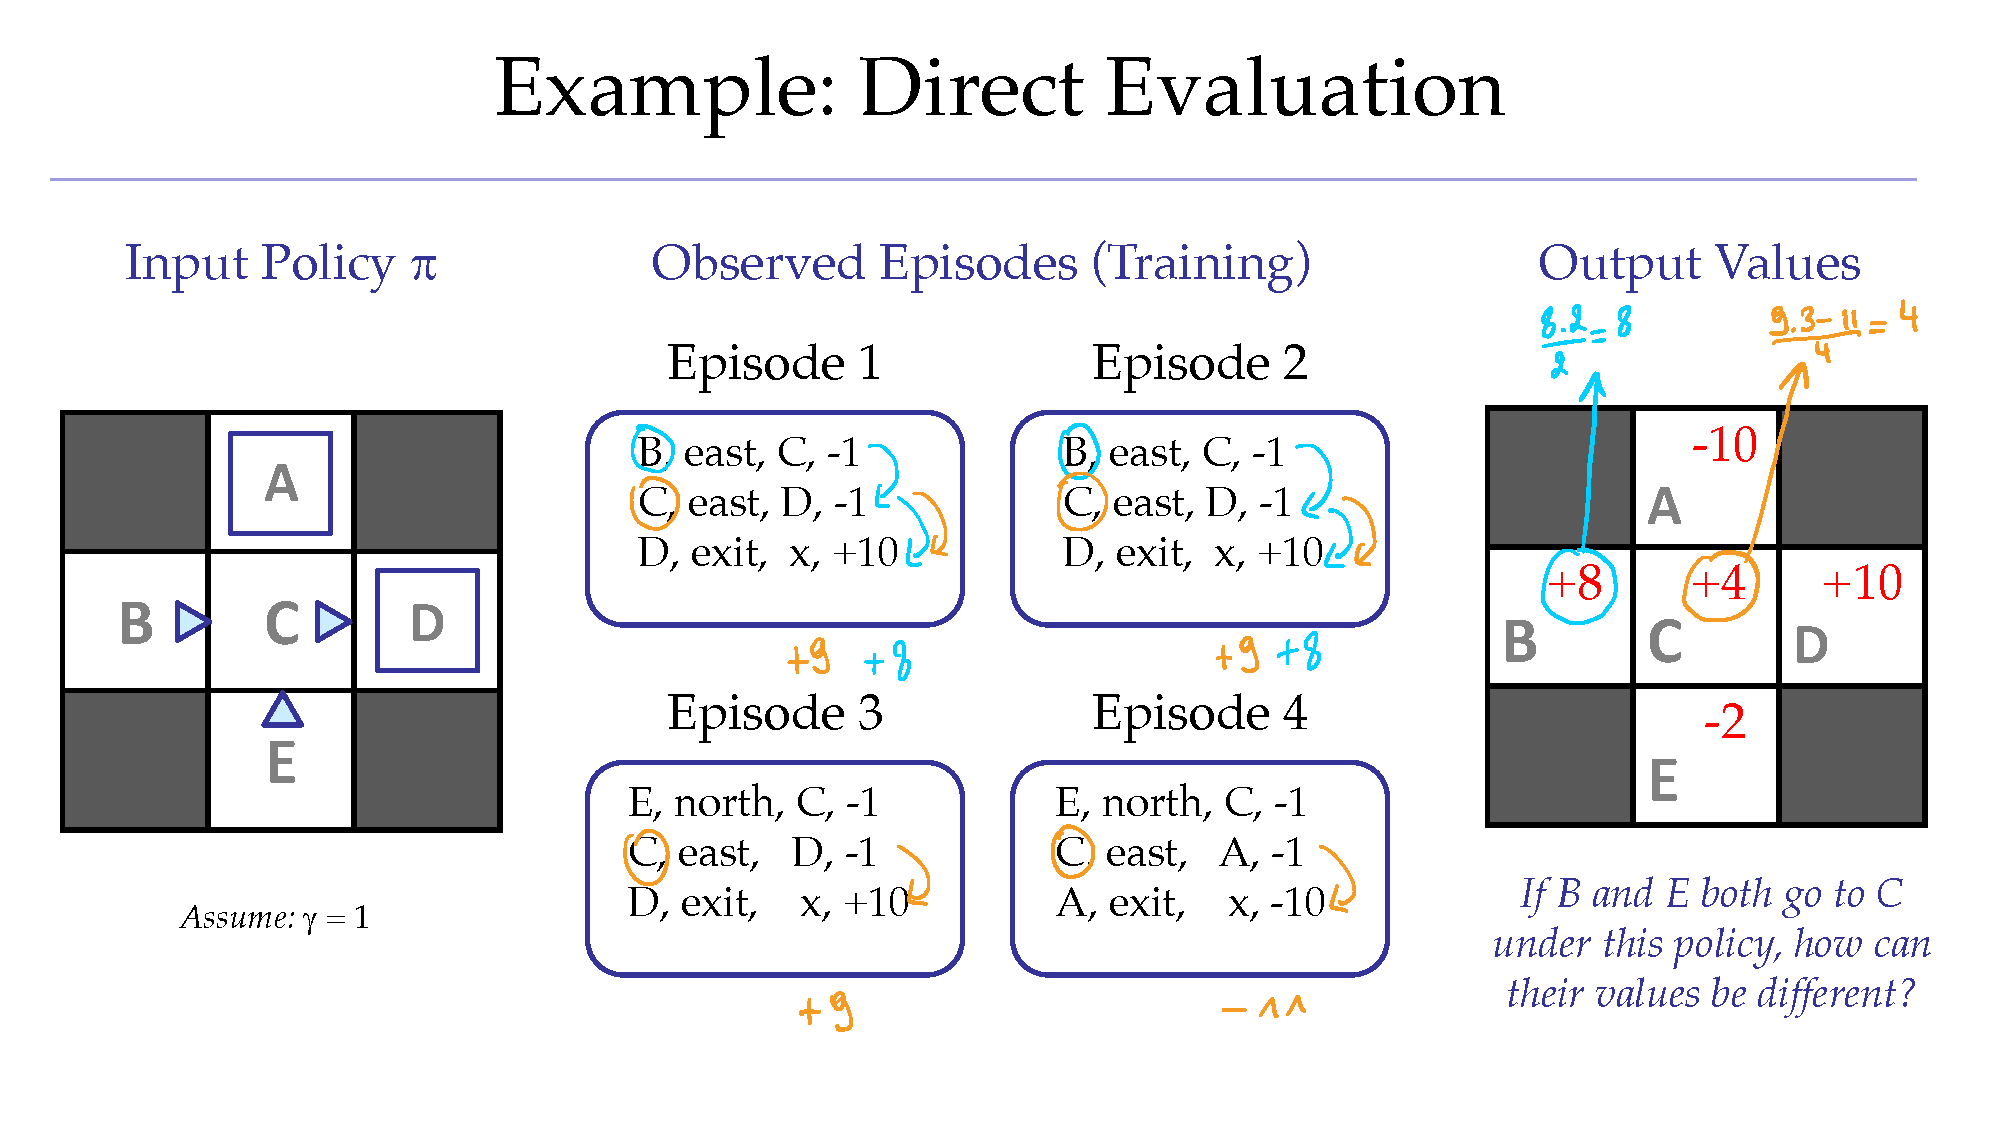
\includegraphics[width=0.7\linewidth]{pictures/example_direct_evaluation.pdf}
        \caption{Exemple de direct evaluation}
        \label{fig:direct_evaluation}
    \end{figure}
\end{example}

Les avantages et les défauts de cette méthode sont les suivants :
\begin{itemize}[label=\textbullet]
    \item[$+$] Simple
    \item[$+$] On a pas besoin de connaitre ni T ni R.
    \item[$+$] Il finitpar calculer les valeurs moyennes correctes en utilisant uniquement les transitions de l'échantillon.
    \item[$-$] Il y a une perte d'information entre les connexions entre les états.
    \item[$-$] Chaque état doit être apppris indépendamment.
    \item[$-$] Il faut beaucoup de temps pour apprendre. 
\end{itemize}

\subsubsubsection{Temporal Difference Value Learning} % (fold)
\label{ssubsub:td_learning}
L'\textbf{idée} est d'apprendre de chaque expérience au fur et à mesure, il faut donc mettre à jour $V(s)$ à chaque fois qu'on
expérimente une transition $(s,a,s',r)$. La politique est toujours fixe mais les valeurs des états vont devenir de plus en plus 
précises. Donc :
 
\begin{itemize}[label=\textbullet]
    \item Sample of $V(s)$: $\text{sample}=R(s,\pi(s),s')+\gamma V^\pi(s')$
    \item Update to $V(s)$: $V(s)\leftarrow (1-\alpha)V^\pi(s)+\alpha\text{ sample}$
    \item En transformant l'équation : $V(s)\leftarrow V^\pi(s)+\alpha(\text{sample}-V^\pi(s))$
\end{itemize}
La dernière équation se lit de la façon suivante, on prend la valeur actuelle de l'état ($V^\pi(s)$) et on ajoute à celle-ci
une petite fraction ($\alpha$) de la différence entre la récompense observée ($\text{sample}$) et la valeur actuelle de l'état
($V^\pi(s)$). De plus, le fait de faire une mise à jour dynamique, nous permet d'aller consulter la valeur de chaque état à tout moment et de la mettre
à jour directement.\\
Le fait de faire une mise à jour de l'interpolation en cours ($\bar{x}_n=(1-\alpha)\cdot\bar{x}_{n-1}+\alpha\cdot x_n$) permet
de rendre les états récents plus importants tandis que les états plus anciens sont moins importants. Si le taux d'apprentissage
$\alpha$ diminue, les moyennes convergent.
\begin{example}
    Voici un exemple de TD learning :
    \begin{figure}[H]
        \centering
        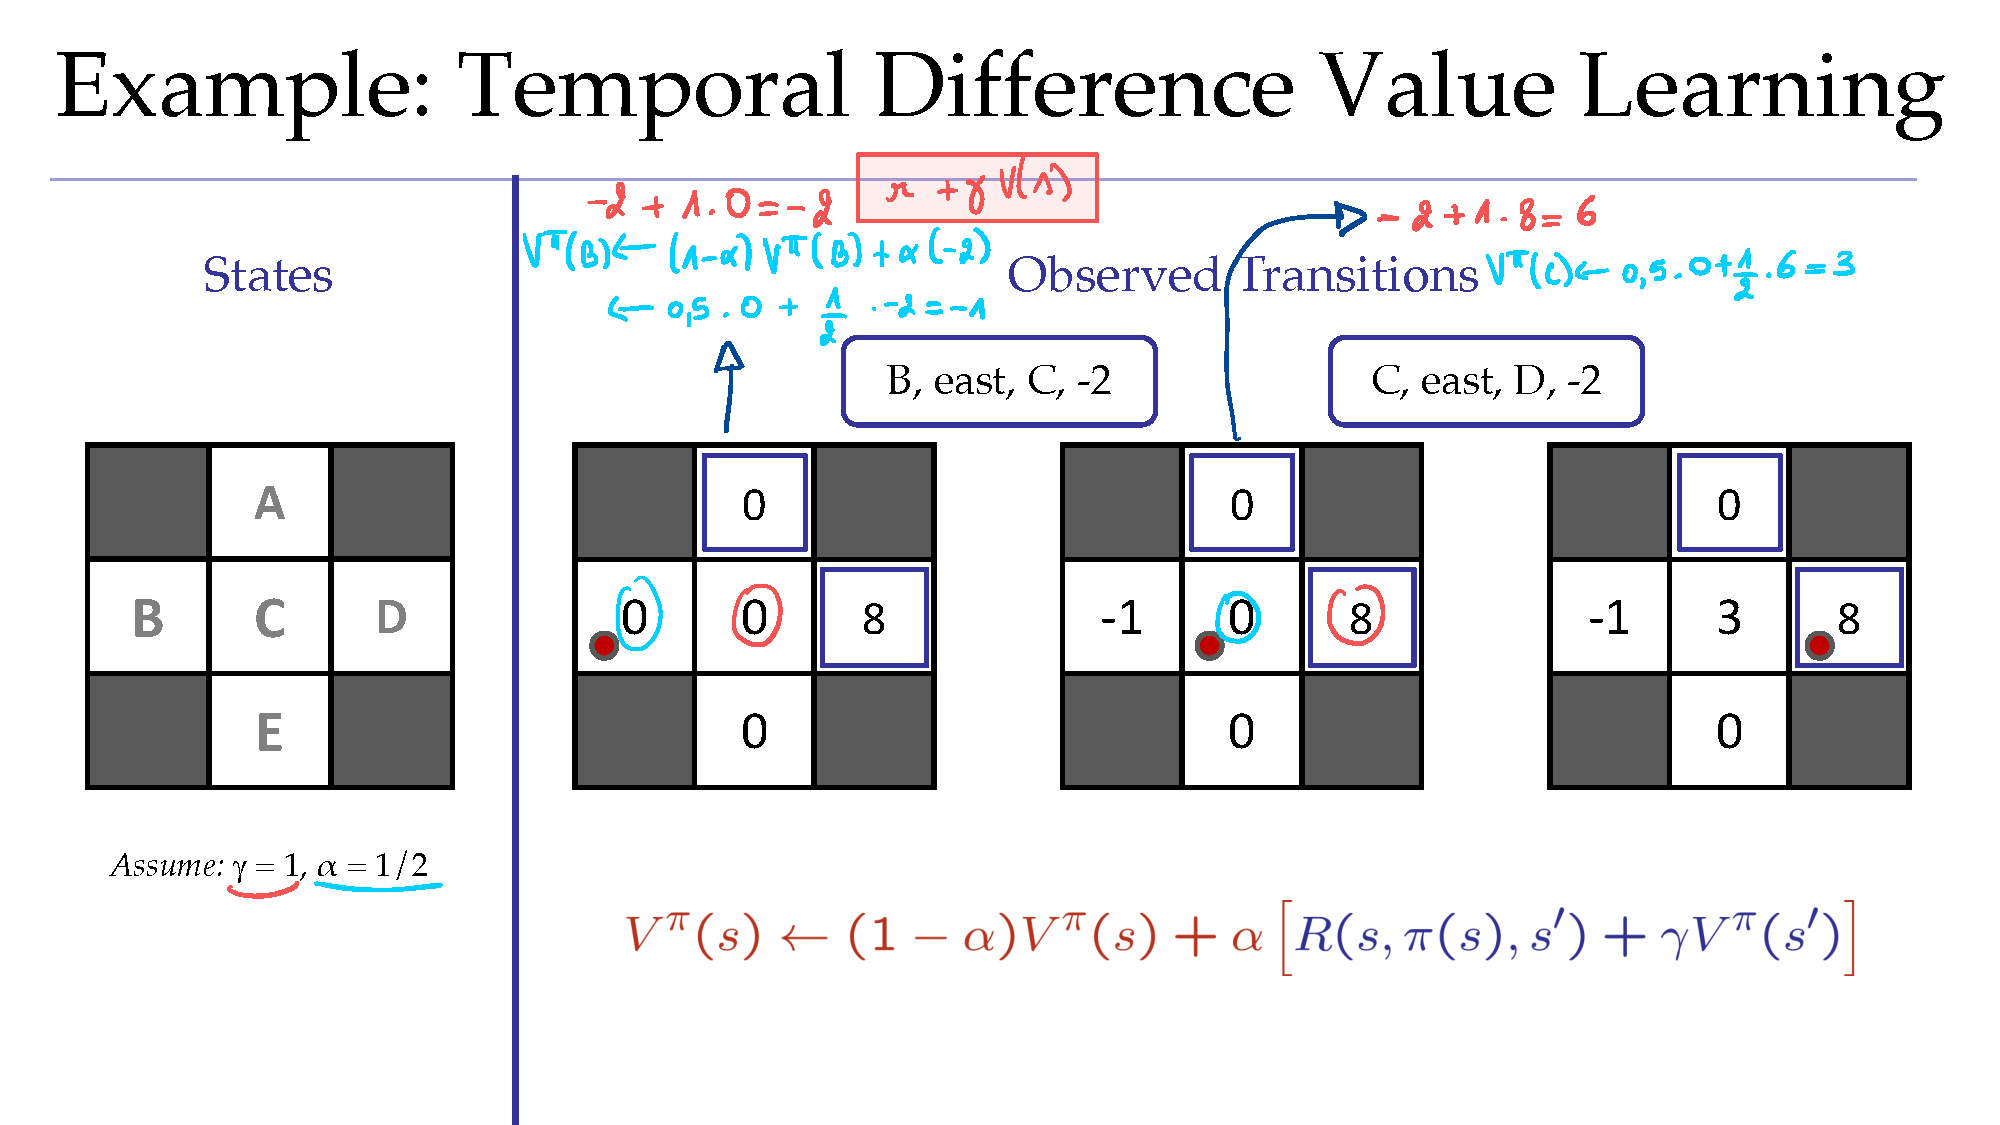
\includegraphics[width=0.7\linewidth]{pictures/example_td_value_learning.pdf}
        \caption{Exemple de TD learning}
        \label{fig:td_learning}
    \end{figure}
\end{example}
Le \textbf{problème} avec le TD learning est que c'est un moyen sans modèle d'évaluer les politiques en imitant les mises à jour
de Bellman avec des moyennes d'échantillons en cours d'exécution. Si on veut transformer les valeurs en une nouvelle politique,
on est perdus, effectivement, on a besoin du modèle pour trouver une nouvelle politique :
\begin{equation*}
    \begin{aligned}
        \pi(s)&=\max\limits_{a} Q(s,a)\\
        Q(s,a)&=\sum_{s'}T(s,a,s')[R(s,a,s')+\gamma V(s')]
    \end{aligned}
\end{equation*}
\subsubsection{Sample-based Policy Evaluation}
Dans le cas où nous sommes dans un état $s$ et qu'en suivant la politique $\pi(s)$, nous arrivons dans un état $s$, et que nous
appliquons à nouveau la politique $\pi(s)$, et depuis cet état on choisit aléatoirement à quel état $s'$ on arrive. Les équations
de Bellman nous permettent de trouver les valeurs des états de façon efficaces :
\begin{equation}
    \begin{aligned}
        V_0^{\pi}(s)&=0\\
        V_{k+1}^{\pi}(s)&=\sum_{s'}T(s,\pi(s),s')[R(s,\pi(s),s')+\gamma V_k^{\pi}(s')]
    \end{aligned}
\label{eq:bellman}
\end{equation}
Dans ce cas, nous exploitons clairement le lien entre les états, mais nous devons connaitre $T$ et $R$.\\
Pour faire sans, nous pouvons prendre un ensemble d'échantillons (en faisant les actions) et en faisant la moyenne.
\begin{equation*}
    \begin{aligned}
        \text{sample}_1 &= R(s,\pi(s),s'_1)+\gamma V^\pi_k(s'_1)\\
        \text{sample}_2 &= R(s,\pi(s),s'_2)+\gamma V^\pi_k(s'_2)\\
        \vdots\\
        \text{sample}_n &= R(s,\pi(s),s'_n)+\gamma V^\pi_k(s'_n)
    \end{aligned}
\end{equation*}
De cette manière nous évaluons l'équation (\ref{eq:bellman}) en utilisant des échantillons. En équation cela donne :
\begin{equation*}
    V_{k+1}^{\pi}(s)\leftarrow\frac{1}{n}\sum_{i=1}^{n}\text{sample}_i
\end{equation*}


\subsection{Active Reinforcement Learning} % (fold)
La différence avec le passive RL est que nous pouvons choisir les actions à prendre. L'apprenant prend désormais des décisions.



\subsubsection{Q-learning} % (fold)
\label{ssubsub:q_learning}
Value iteration trouve des valeurs successives (limitées par une profondeur max) mais les \textbf{Q-values} sont plus pratiques, 
nous pouvons réécrire les équations de value iteration ($V_{k+1}(s)=\max\limits_{a}\sum_{s'}T(s,a,s')[R(s,a,s')+\gamma V_k(s')]$)
en termes de Q-values :
\begin{itemize}[label=\textbullet]
    \item On commence avec $Q_0(s,a)=0$.
    \item Pour un $Q_k$ donné, on calcule $Q_{k+1}$ pour tous les q-états :
    \begin{equation*}
        Q_{k+1}(s,a)\leftarrow\sum_{s'}T(s,a,s')[R(s,a,s')+\gamma\max\limits_{a'}Q_k(s',a')]
    \end{equation*}
\end{itemize}
La différence entre les deux est que dans le cas des q-values, on commence par une moyenne tandis que dans le cas de value iteration,
on commence par un max. L'utilisation d'échantillons n'est donc pas possible dans value iteration. Sauf qu'avec les q-values,
c'est possible, l'équation écrite au dessus représente en fait la \textbf{Q-value iteration}.\\
A partir d'un échantillon $(s,a,s',r)$, on peut mettre à jour $Q(s,a)$ :
\begin{equation}
    \text{sample} = R(s,a,s')+\gamma\max\limits_{a'}Q(s',a')
    \label{eq:q_value}
\end{equation}
On voit qu'on a plus d'évaluation de politique. On peut intégrer la nouvelle estimation dans la moyenne dynamique :
\begin{equation*}
    Q(s,a)\leftarrow (1-\alpha)Q(s,a)+\alpha\text{ sample}
\end{equation*}
Voici les propriétés de Q-learning :
\begin{itemize}[label=\textbullet]
    \item Q-learning converge vers les Q-valeurs optimales même si on agit de manière suboptimale.
    \item C'est une méthode d'apprentissage "off-policy"
\end{itemize}
Cependant, il faut faire attention à:
\begin{itemize}[label=\textbullet]
    \item Parcourir suffisament longtemps.
    \item Il faut parfois donner une valeur très petite à $\alpha$ mais il ne faut pas le diminuer trop rapidement.
    \item Il n'y a pas vraiment d'importance à la façon dont on choisit les actions.
\end{itemize}
\begin{remark}
    Voici ce qui a été vu jusque maintenant :
    \begin{figure}[H]
        \centering
        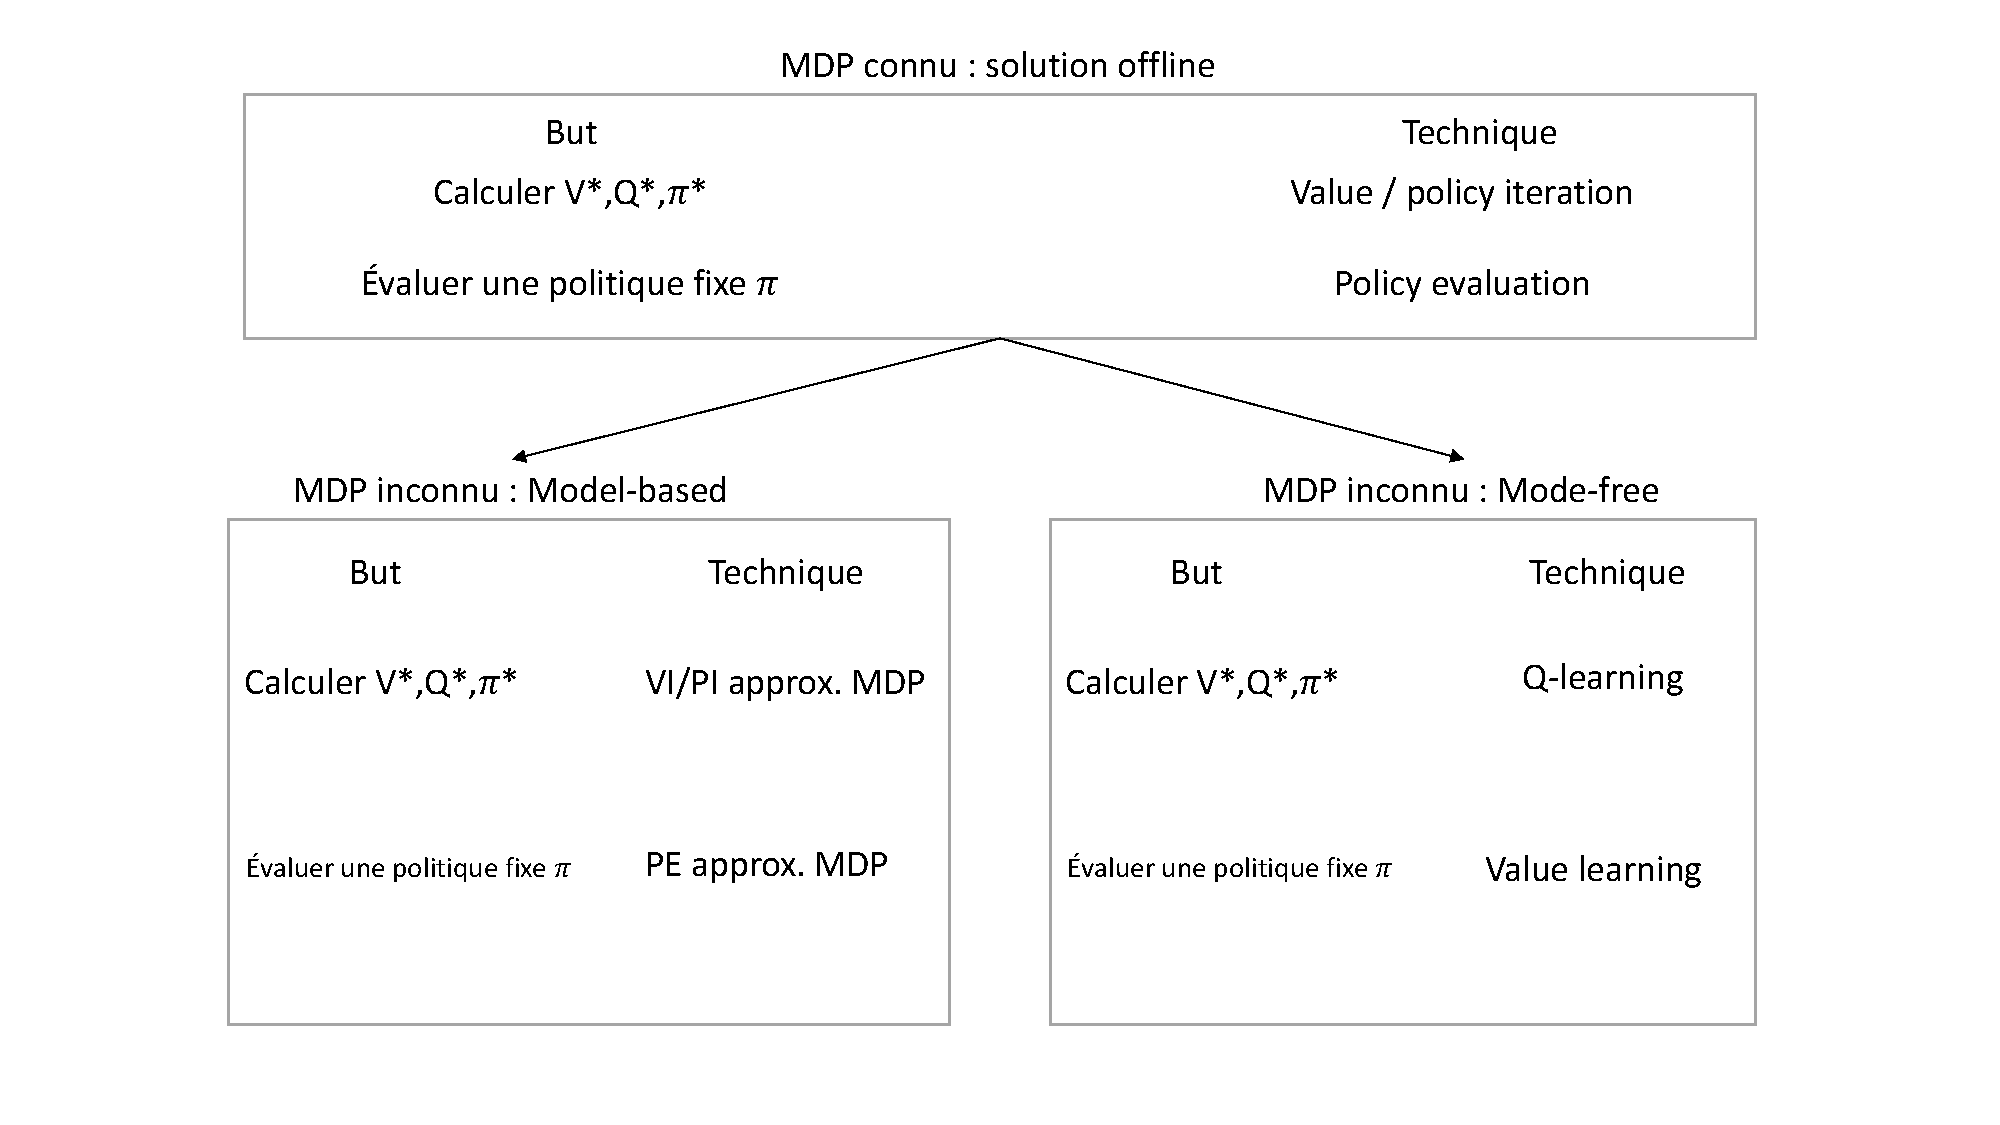
\includegraphics[width=\linewidth]{pictures/resume_offline_RL.pdf}
        \caption{Résumé de ce qui a été vu jusque maintenant}
        \label{fig:rl_summary}
    \end{figure}
\end{remark}

\subsection{Exploration vs Exploitation} % (fold)
\label{sub:exploration_vs_exploitation}
\begin{example}
    Imaginons que vous alliez toujours dans le même restaurant qui est très bien et que vous adorez y aller. Mais un jour,
    un tout nouveau restaurant ouvre juste à côté, est-ce que vous aller continuer à aller dans le même restaurant ou est-ce
    que vous allez essayer le nouveau restaurant ? Aller tester le nouveau restaurant est risqué car il pourrait être moins
    bon que l'ancien. C'est le dilemme entre l'exploration et l'exploitation.
\end{example}

\subsubsection{$\epsilon$-greedy} % (fold)
C'est le plus simple, on choisit entre prendre une action aléatoire (avec une probabilité de \textbf{$\epsilon$}) ou alors 
suivre la politique (avec une probabilité, plus élevée, de \textbf{$1-\epsilon$}).\\
Dans ce cas, si l'algorithme tourne suffisament longtemps, nous sommes sûrs d'explorer tous les états et les q-values vont
converger vers les valeurs optimales. Afin d'avoir ces valeurs optimales, il faut que le $\epsilon$ diminue dans le temps afin
de converger vers une politique optimale.
 
\subsubsection{Fonctions d'exploration} % (fold)
L'idée ici se base (plutôt que d'explorer de façon aléatoire) sur le fait d'explorer des états qui sont pas encore bien connus.
Mais si on connait bien un état, cela ne sert à rien de revisiter cet état.\\
Pour ce faire, on utilise une fonction d'exploration de la forme suivante : $f(u,n)=u+\frac{k}{n}$ où $u$ est la valeur de
l'état et $n$ est le nombre de fois qu'on a visité l'état et $k$ est une constante. Nous remarquons donc qu'au plus un état
a été visité, la fonction diminue puisque le terme en $\frac{k}{n}$ diminue ($n>>$).\\
La q-value de l'équation (\ref{eq:q_value}) s'écrit désormais :
\begin{equation*}
    Q(s,a) \leftarrow_{\alpha} R(s,a,s')+\gamma\max\limits_{a'}f(Q(s',a'),N(s',a'))
\end{equation*}
Où $\leftarrow_{\alpha}$ dit qu'on fait une mise à jour avec un poids, on a déjà une valeur Q, on en a une nouvelle et donc on
va combiner \textbf{l'ancienne $+(\alpha\times)$ la nouvelle}. Dès lors, on prend en compte les états qui n'ont pas été visité
beaucoup en leur donnant une valeur plus élevée, si on a des actions dans $s'$ qu'on a pas encore beaucoup prises, si c'est le
cas, alors la valeur sera plus grande.

\subsubsection{Regret} % (fold)
Si on a appris deux politiques optimales selon deux algorithmes différents, comment savoir laquelle est la meilleure ?\\
Il faut prendre en compte non seulement la récompense finale mais on va regarder toutes les récompenses obtenus au fur 
et à mesure de l'algorithme. On regardera par exemple quel algorithme a trouvé la politique optimale de façon la plus rapide.
La notion de regret intervient dans cette comparaison, et donc une exploration aléatoire aura un regret bien plus élevé qu'une
exploration basée sur des fonctions d'exploration. Le regret ne sera jamais égal à 0.
\begin{figure}
    \centering
    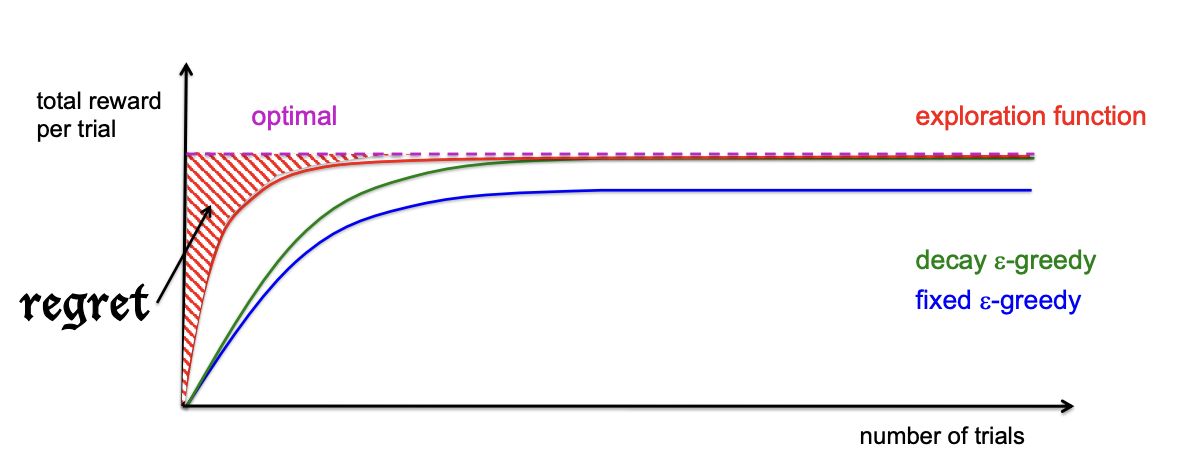
\includegraphics[width=0.7\linewidth]{pictures/regret.png}
    \caption{Exemple de regret}
    \label{fig:regret}
\end{figure}

\subsection{Approximate Q-learning} % (fold)
Dans le cas de q-learnin, on garde une table avec toutes les q-values. Cependant, dans des situations réalistes, on ne peut pas
faire ceci, car trop d'états par exemple. Le but est d'apprendre d'un nombre d'état minimum et d'ensuite faire une généralisation.
\begin{example}
    Si on a déjà été dans un building par une certaine porte, on peut essayer d'entrer dans un autre building même si on ne 
    connait pas et qu'on a jamais vu la porte de ce nouveau building.
\end{example}

La solution c'est de décrire un état par un vecteur de features (propriétés). Pour combiner les valeurs de ces features, on 
va utiliser des fonctions de valeur linéaires. On pourrait faire ceci sur le value learning ou sur le q-learning mais ici, on
va se concentrer sur le q-learning :
\begin{equation}
    Q(s,a)=w_1f_1(s,a)+w_2f_2(s,a)+\dots+w_nf_n(s,a)
    \label{eq:approx_q_learning}
\end{equation}
Donc ici, on a un ensemble de features ($f_1,f_2,\dots,f_n$) et un ensemble de poids ($w_1,w_2,\dots,w_n$). On attend de q-learning
d'apprendre ces poids, de façon qu'une fois que les poids sont appris, les q-values soient plus ou moins optimales.
\warningbox{
    Il se peut que deux états aient les mêmes features mais des q-values différentes.
}
Pour une transition $(s,a,r,s')$, on a la différence qui vaut $[r+\gamma\max\limits_{a'}Q(s',a')]-Q(s,a)$. Dès lors :
\begin{equation*}
    \begin{aligned}
        Q(s,a) &\leftarrow Q(s,a)+\alpha[\text{différence}]\\
        w_i &\leftarrow w_i+\alpha[\text{différence}]f_i(s,a)
    \end{aligned}
\end{equation*}
\begin{example} Voici un exemple sur le jeu Pac-Man :
    \begin{figure}[H]
        \centering
        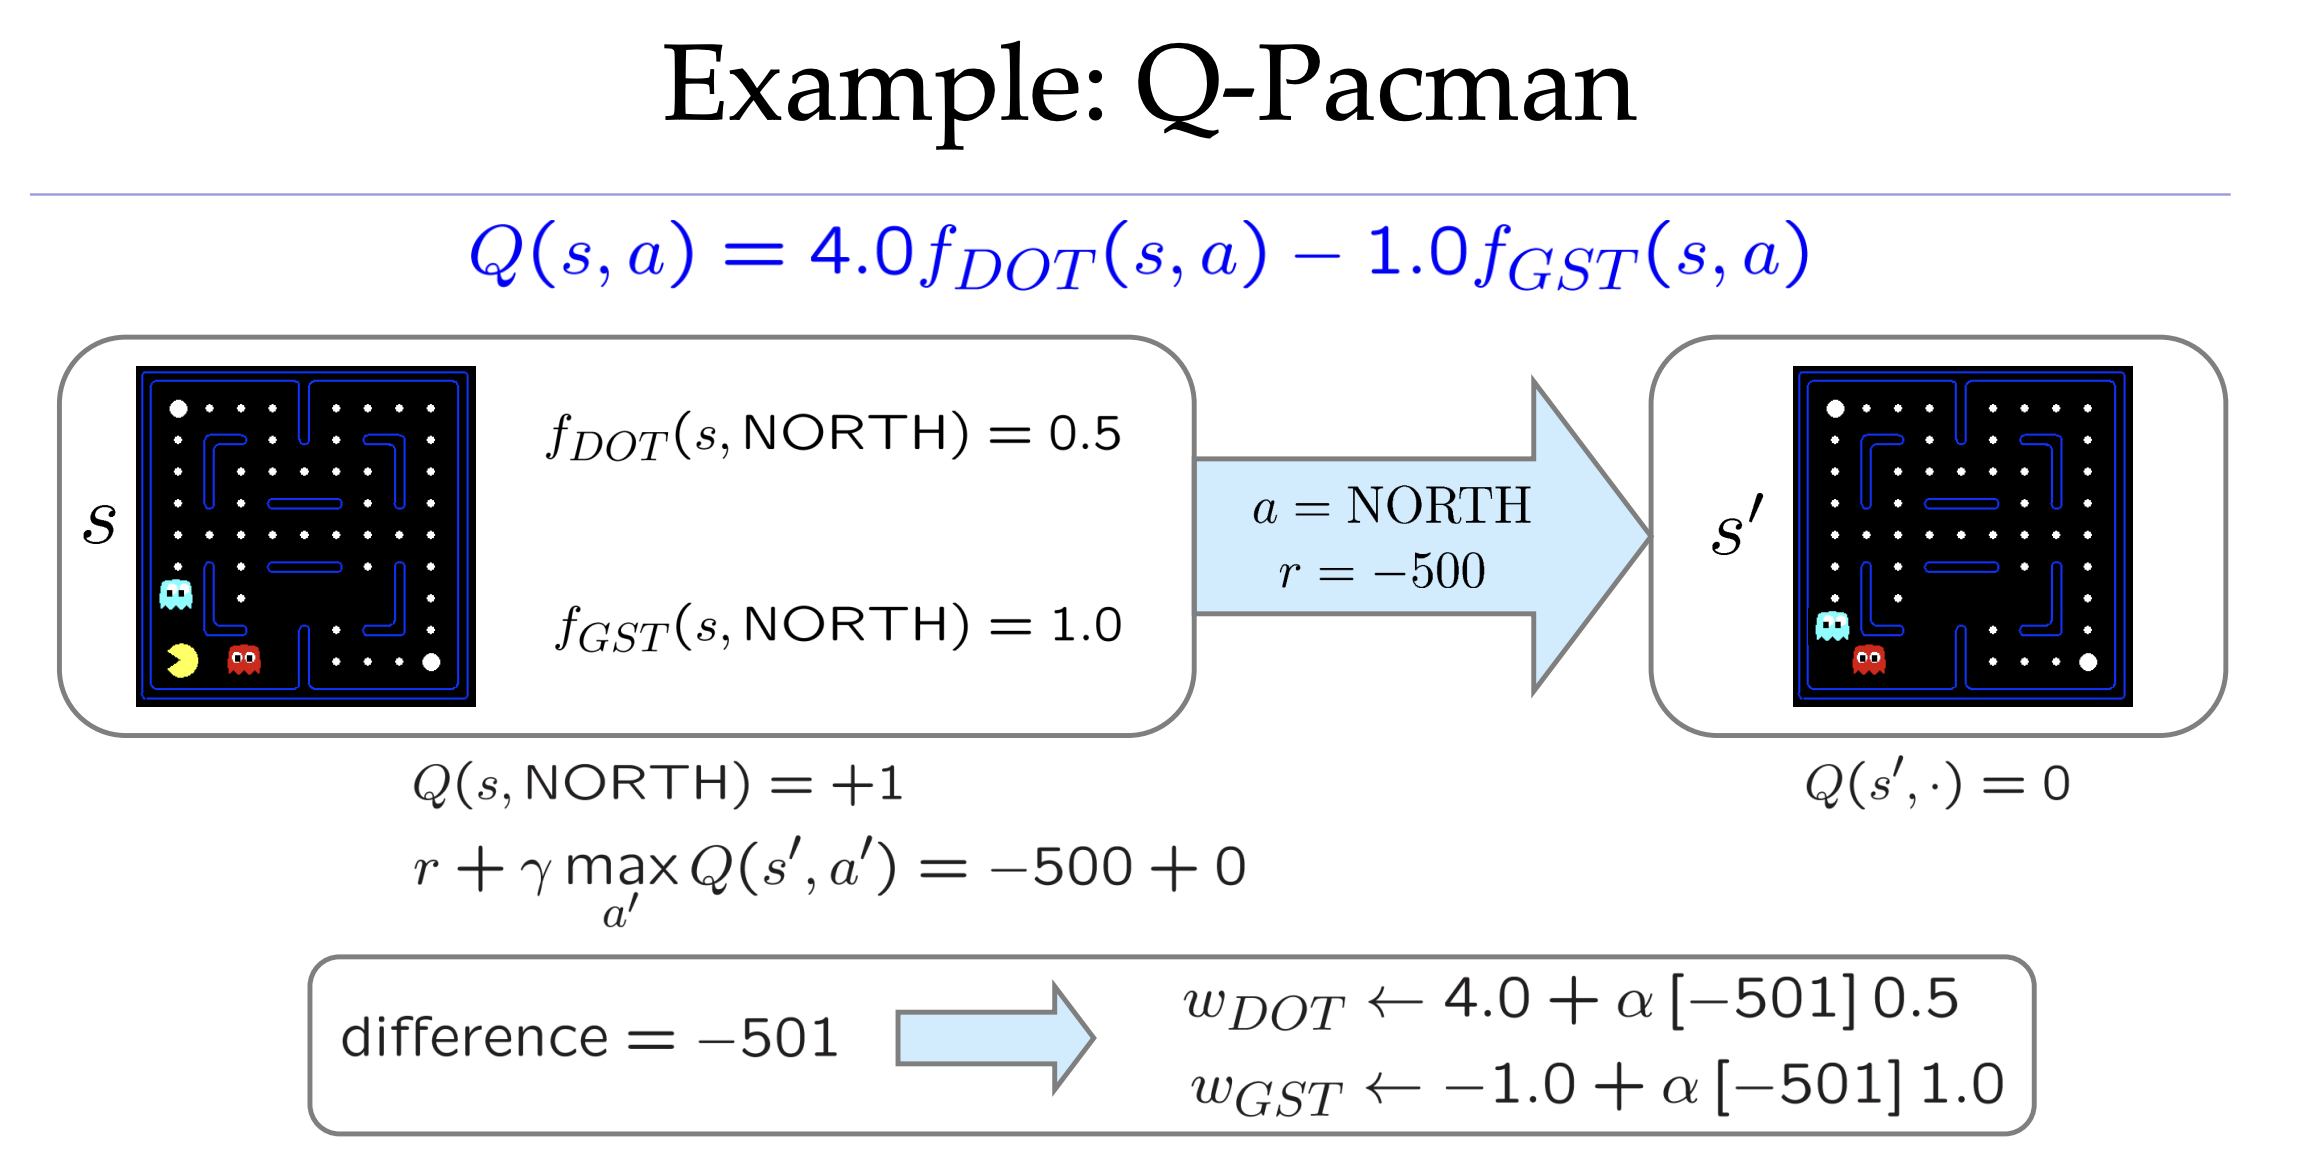
\includegraphics[width=0.7\linewidth]{pictures/q-pacman.png}
        \caption{Exemple d'approximate q-learning}
        \label{fig:approx_q_learning}
    \end{figure}
    Avec $f_{DOT}$ qui est le feature du joueur par rapport à un point et $f_{GST}$ qui est le feature du joueur par rapport à un
    fantôme.\\
\end{example}